\documentclass[12pt]{elsarticle}
\usepackage[top=40mm,bottom=40mm,left=30mm,right=30mm]{geometry}
\usepackage[brazil]{babel}
\usepackage[utf8x]{inputenc}
%\usepackage[latin1]{inputenc}
\usepackage{ae}
\usepackage{indentfirst}
\usepackage{url,multirow}
\usepackage{colortbl}
\usepackage{amssymb,amsmath}
\usepackage{dsfont}
\usepackage{float}
\usepackage[dvipsnames]{xcolor}
\usepackage{rotating}
\usepackage[ruled,vlined,linesnumbered,portuguese]{algorithm2e}
\usepackage{soul}
\usepackage[noend]{algpseudocode}
\usepackage{threeparttable}
\usepackage{caption}
\usepackage{subcaption}
\usepackage{listings}
\usepackage{color}
\usepackage{tkz-graph}
\usepackage{todonotes}
\usepackage[hidelinks]{hyperref}
\usepackage{algpseudocode}
\usepackage{framed}
\newtheorem{mytheo}{Teorema}
\newtheorem{mylem}{Lemma}[mytheo]
\newtheorem{mycor}{Corollary}[mytheo]
\newenvironment{definition}[1][Poligonização de Área Máxima:]{\begin{trivlist}\setlength{\leftskip}{18pt}
		\item[\hskip \labelsep {\bfseries #1}]}{\end{trivlist}}
\newenvironment{proof}{\noindent{\bf Proof:}}{\null\hfill $\rule{1.5mm}{1.5mm}$}
\addtolength{\abovecaptionskip}{-7mm}
\newcommand{\HRule}{\rule{\linewidth}{0.5mm}}

\newcommand\mycommfont[1]{\footnotesize\ttfamily\textcolor{ForestGreen}{#1}}
\SetCommentSty{mycommfont}
\presetkeys{todonotes}{inline}{}

\selectlanguage{brazil}

\graphicspath{{figuras/}}


\lstset{
	numbers=left,
	frame=single,
	framexleftmargin=1.5em,
	language=Python,
	showstringspaces=false,
	columns=flexible,
	basicstyle={\small\ttfamily},
	breaklines=true,
	breakatwhitespace=true,
	tabsize=3
}

\begin{document}
	
	\pagenumbering{roman}
	
	\hyphenation{con-su-mi-dor com-pa-ran-do-os}
	
	\selectlanguage{brazil}
    
    \title{Algoritmo Evolutivo para o Problema de Distritamento-Roteamento}
	
	\begin{titlepage}
	\begin{center}
		% Upper part of the page
		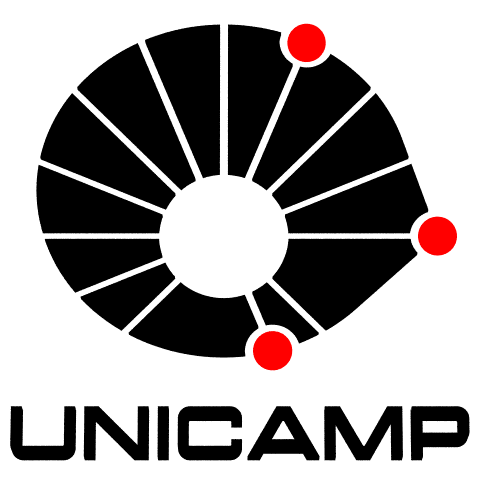
\includegraphics[width=0.15\textwidth]{LogoUnicamp.png}\\[1cm]
		\textsc{\large Universidade Estadual de Campinas}\\[0.25cm]
		\textsc{\large Faculdade de Engenharia Mecânica}\\[2.0cm]
		\textsc{\Large Trabalho de Graduação - Relatório Parcial} \\ [2.0cm]
		\HRule \\[1.5cm]
		{ \bfseries \Large Algoritmo Evolutivo para o Problema de Distritamento-Roteamento}\\[1.5cm]
		{ \bfseries \Large Evolutionary Algorithm for the Districting-Routing Problem}\\[1.5cm]
		\HRule %\\[1.5cm]
		
		\vfill
		
		% Author and supervisors
		\newcolumntype{R}{>{\raggedleft\arraybackslash}X}
		\newcolumntype{L}{>{\raggedright\arraybackslash}X}
		\large \emph{Aluno: Davi Rodrigues} \\
		\large \emph{Orientador: Prof. Dr. Fábio Luiz Usberti}\\
		
		\vfill
		% Bottom of the page
		{\large Abril - 2017}
	\end{center}
\end{titlepage}
	
	\newpage
	
	\renewcommand{\contentsname}{\centering Sumário}
	\tableofcontents
	
	\newpage
	\phantomsection
	\addcontentsline{toc}{section}{Resumo}
	
	\setcounter{page}{1}
	\pagenumbering{arabic}
	
	\begin{center}
		\textbf{Resumo} \label{sec:Resumo}
	\end{center}
    
	O problema do caixeiro-viajante (TSP) propõe encontrar o menor caminho possível para se percorrer um grafo $G=(V,E)$, visitando todos os nós $V$ através de suas arestas $E$, das quais a cada uma é atribuído um custo. Uma generalização do TSP é o problema de distritamento-roteamento, onde o objetivo é particionar o grafo em um número pré-determinado de distritos conexos, onde cada distrito será percorrido por um veículo próprio, de forma a se obter o menor caminho total. O objetivo deste trabalho é propor uma metodologia de solução para o problema distritamento-roteamento através de uma meta-heurística baseada em algoritmos evolutivos. Espera-se avaliar o desempenho da solução meta-heurística a partir de experimentos computacionais utilizando instâncias geradas aleatoriamente.


	
	\begin{center}
		\textbf{Abstract} \label{sec:Abstract}
	\end{center}
    
	The travelling-salesman problem (TSP) proposes to find the smallest possible way to go through a graph $G = (V, E)$, visiting all nodes $V$ through their edges $E$, of which each one is assigned a cost. A generalization to the TSP is the districting-routing problem, where the goal is to partition the graph into a predetermined number of related districts, where each district will be driven by its own vehicle, in order to obtain the smallest total path. The objective of this work is to propose a solution methodology for the districting-routing problem through a metaheuristic based on evolutionary algorithms. It is expected to evaluate the performance of the metaheuristic solution from computational experiments using randomly generated instances.
	
	\newpage
    
    %%%%%%%%%%%%%%%%%%%%%% INTRODUÇAO %%%%%%%%%%%%%%%%%%%%%
    
	\section{Introdução} \label{sec:Introducao}
    
    \subsection{Conceitos introdutórios}
    
    Um grafo dito direcionado $G = (V,E,(s,t))$ consiste de um conjunto de vértices (nós) $V$, um conjunto de arestas (arcos) $E$, e uma função $(s,t) : E \rightarrow V$, onde $s(e)$ é a fonte e $t(e)$ é o alvo da aresta direcionada $e$. Um grafo é dito não-direcionado quando, ao invés da função $(s,t) : E \rightarrow V$, possui uma função $w : E \rightarrow P(V)$ que associa cada aresta a um subconjunto de até dois elementos de $V$, sendo estes os pontos terminais da aresta. Um grafo com pesos possui uma função adicional $E \rightarrow R$ que associa um valor (custo) a cada aresta.
    
    O grau de um vértice é definido como o número de arestas incidentes a ele. Caso haja um laço no vértice é considerado as suas duas extremidades no cálculo do grau. Um laço é definido como uma aresta cuja duas extremidades incidem no mesmo nó.
    
    Um passeio $p=(v_0,v_k)$ em um grafo é uma lista de vértices e arestas que inicia no vértice $v_0$ e termina no vértice $v_k$, em que cada dois vértices consecutivos são ligados por uma aresta. Ou seja, um passeio é uma sequencia $<v_0, a_1, v_1, a_2, ... , v_{k-1}, a_k, v_k>$ onde $v_0, v_1, ... , v_k$ são vértices e $a_1, ... , a_k$ são arestas e, para cada $i$, $a_i$ é um arco de $v_{i-1}$ a $v_i$. Um caminho é um passeio onde não existem vértices repetidos. Um passeio é dito ciclo quando $v_0 = v_k$
    
    Um caminho ou ciclo é dito euleriano se utiliza cada uma de suas arestas uma vez. Um caminho ou ciclo é dito hamiltoniano se utiliza cada um dos seus vértices uma vez.
    
    O custo de um caminho ou ciclo é definido como $\sum_{i=1}^{i=k}r_i$, onde $r_i$ é o custo associado à aresta $a_i$.
    
    \subsection{Problema de Distritamento e Roteamento}
    
    O problema de distritamento e roteamento (em inglês \textit{districtiong and routing problem} - DRP) é uma generalização do problema do caixeiro-viajante (em inglês \textit{traveling salesman problem} - TSP). O TSP consiste na busca de um ciclo hamiltoniano com o menor custo possível. O espaço de busca aumenta fatorialmente em relação ao número de nós, tornando a busca por uma solução exata impraticável para instâncias suficientemente grandes, sendo que um grafo com $n$ nós possui $\frac{(n-1)!}{2}$ ciclos hamiltonianos \cite{agarwal}. 
    
    No DRP buscamos dividir o grafo em um número pré-determinado de distritos conexos, onde cada distrito será percorrido por um “caixeiro” (veículo) próprio. O DRP pode ser modelado como um grafo não-direcionado $G=(V,E)$, onde $V = \{v_0\} \cup V^*$, sendo $V^*$ o conjunto de clientes, $\{v_0\}$ o conjunto de depósitos, de onde os veículos devem partir e retornar; e $E = \{(v_i, v_j): v_i,v_j \in V, i<j\}$ é o conjunto de arestas \cite{wang}. Dependendo da aplicação, diferentes objetivos podem ser considerados para a otimização, como, por exemplo, número de distritos, somatório dos custos dos trajetos dos veículos, equilíbrio de trabalho entre os veículos, compacidade dos distritos, deadhead (caminho percorrido sem realizar trabalho), lucro gerado pelos veículos, entre outros.
    
\begin{figure}[H]
\centering
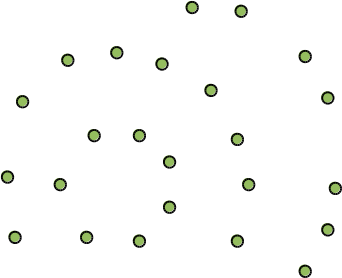
\includegraphics[width=0.7\textwidth]{grafo.png}
\vspace{0.5cm}
\caption{\label{fig:proporcionalreaposta}Vértices de um grafo}
\end{figure}

\begin{figure}[H]
\centering
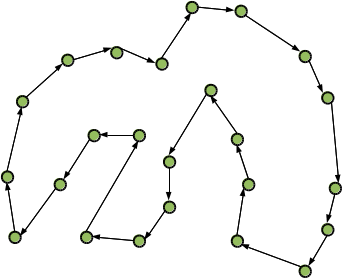
\includegraphics[width=0.7\textwidth]{grafo-distrito1.png}
\vspace{0.5cm}
\caption{\label{fig:proporcionalreaposta}Caminho hamiltoniano}
\end{figure}

\begin{figure}[H]
\centering
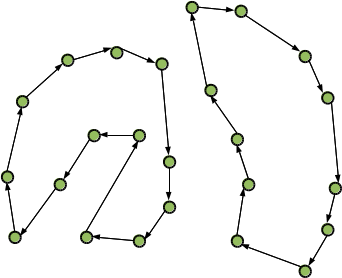
\includegraphics[width=0.7\textwidth]{grafo-distrito2.png}
\vspace{0.5cm}
\caption{\label{fig:proporcionalreaposta}Caminho hamiltoniano dividido em dois distritos}
\end{figure}

\begin{figure}[H]
\centering
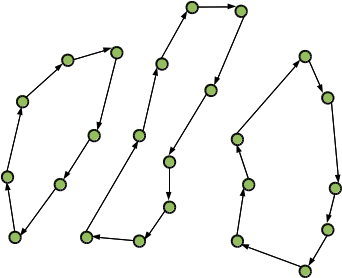
\includegraphics[width=0.7\textwidth]{grafo-distrito3.png}
\vspace{0.5cm}
\caption{\label{fig:proporcionalreaposta}Caminho hamiltoniano dividido em três distritos}
\end{figure}
    
    
    \subsection{Aplicação Prática}
    
    O DRP possui similaridades com diversos problemas de aplicação prática, como supply chain, serviços de entregas, localização de centros de distribuição, serviços de mobilidade urbana, correios, etc. \cite{groer} \cite{wang}
    
    %%%%%%%%%%%%%%%% TRABALHOS RELACIONADOS %%%%%%%%%%%%%%%%
	
	\section{Trabalhos Relacionados} \label{trabalhosRelacionados}
	
	\subsection{Problema Dinâmico de Locação-Roteamento de Veículos} \label{locationRouting}
    O problema dinâmico de locação-roteamento (DLRP) pode ser dividido em duas partes: o problema de alocação de localização (LAP), que visa buscar os melhores pontos de partida (depósitos) para um grafo dividido em distritos; e o problema de roteamento de veículos (VRP), que trata de uma generalização do TSP, onde vários veículos percorrem o grafo. A natureza dinânica do problema se dá no fato do grafo ser mutável, com novos nós e arcos surgindo no decorrer do tempo. Os algoritmos de colonia de formigas são uma alternatida de meta-heurística para a resolução deste problema. Tang et al. mostraram que um algoritmo de clusterização associado com um algoritmo de colônia de formigas (KACO) tem melhor desempenho e mesmo custo computacional aproximado em relação a algoritmos de colonia de formigas sem cluterização (WKACO) \cite{tang}, utilizando de diferentes métodos de formigas imigrantes para lidar com a natureza dinâmica do problema.
	
	\subsection{Problema Dimânico e Multi-Objetivo de Distritamento e Roteamento Estocástico} \label{districtingAndRouting}
    Laport et al. \cite{wang} apresentam o Problema Dinâmico e Multi-Objetivo de Distritamento e Roteamento Estocástico (MDSDRP), onde existem duas classes de clientes: os regulares, de localização conhecida, e os estocásticos, que surgem e desaparecem de maneira aleatória ao longo do tempo e possuem localização e presença incertas. O problema é modelado como um grafo $G=(V,E,P)$, onde $P$ é o conjunto de períodos, $V$ é a união dos conjunto de vertices, conjunto de depósitos (pontos de partida e chegada dos veículos), e o conjunto de clientes em cada período, e $E$ é a matriz que define os custos e tempos de viagem entre os vértices. Com caráter multi-objetivo, espera-se otimizar vários fatores além dos custos totais, como: minimizar quantidade de distritos, gerar distritos compactos, lucro gerado por veículo, etc. Para lidar com este problema, os autores utilizam algoritmos evolutivos não só para buscar a melhor forma de distritamento, mas também para evoluir o vetor de objetivos. 
    
    \subsection{Problema de Distritamento no Contexto de Roteamento de Arcos}
    Diferente dos casos citados anteriormente, no Arc Routing Problem (ARP), o objetivo é percorrer um determinado subconjunto de arcos em um grafo ao invés de visitar nós. Este problema modela diversas situações reais, como coleta de lixo, entrega de correspondencias, manutenção pública, etc. 
    
    Prins et al. \cite{prins} comparam três métodos heurísticos para a solução do ARP com setoreamento de arcos (SARP). O primeiro, \textit{circuit of tasks heuristic} (CTH) é uma heurística em duas fases (TPH), cuja primeira fase busca determinar os setores e a segunda fase busca calcular as rotas dentro de cada setor. No CTH, o objetivo é calcular um circuito de demanda minima em um grafo balancedo e atribuir todas as tarefas deste circuito a um setor, no qual as tarefas possam ser associadas a um pequeno conjunto de arcos durante a fase de roteamento. O segundo algoritmo, \textit{single task heuristic} (STH), também é um TPH, mas, diferente do CTH, os setores crescem adicionando-se uma tarefa por vez. O terceiro algoritmo utilizado, \textit{best insertion heuristic}, constrói rotas e setores concomitantemente.
    
    %Laport et al. \cite{laporte} propõe uma meta-heuristica para o ARP utilizando uma otimização de dois estágios a partir de uma solução inicial, combinando busca tabu e pesquisa de vizinhança randomizada e adaptativa. Como a vizinhança de uma solução pode ser muito grande, sub-rotinas baseadas em busca tabu são utilizadas para restringir o espaço de busca de novas soluções. Para a busca da solução inicial é utilizado o algoritmo de particionamento recursivo (RPA) com uma etapa de pós-processamento para garantir a continuidade de cada partição.
    
    Um novo critério de otimização é introduzido por Fernández et al. \cite{fernandez}. Além dos critérios típicos, como continuidade e compacedade dos distritos, balanceamento do custo e o deadhead (distancia percorrida sem realizar trabalho), também é considerado a paridade dos distritidos. Paridade é definida como o critério que penaliza partições de arcos que possuem grau ímpar de nós em seus subgrafos.

	%%%%%%%%%%%%%%%%%%%%%% OBJETIVOS %%%%%%%%%%%%%%%%%%%%%

	\section{Objetivos}  \label{sec:objetivos}
	
    Este trabalho tem por objetivo propor, implementar e analisar metodologias heuristicas baseadas em algoritmos genéticos para a solução do Problema de Distritamento-Roteamento (DRP).
    
	\subsection{Objetivos Gerais} \label{sec:objetivosGerais}
    
    \begin{itemize}
    
    \item Propor um método heurístico baseado em algoritmo genético para a solução do DRP.
    \item Criar instancias para o DRP.
    \item Realizar avaliação dos metodos desenvolvidos.
    
    \end{itemize}
    
    
	
	\subsection{Objetivos Específicos} \label{sec:objetivosEspecificos}
    
    \begin{itemize}
    \item Propor e implementar uma meta-heurística para a solução do problema baseada em Algoritmos Genéticos.
    \item Delimitar parâmetros de otimização.
    \item Definir parâmetros para o algoritmo genético.
    \item Criação de instâncias de tamanhos variados para o problema.
    \item Realizar experimentos computacionais para a comparação da qualidade das soluções dos métodos propostos.
    \end{itemize}
	
    %%%%%%%%%%%%%%%%%%%%% METODOLOGIA %%%%%%%%%%%%%%%%%%%%%%
    
	\section{Metodologia} \label{metodologia}
    
    \subsection{Algoritmos genéticos}
    
    Devido à complexidade dos problemas NP-difíceis como o TSP e o DRP, ainda não são conhecidos algoritmos exatos que fornecem uma solução ótima em tempo polinomial. Por outro lado, existem outras metodologias de solução denominadas meta-heurísticas que na prática apresentam bom desempenho, fornecendo soluções próximas ao ótimo. Dentre as meta-heurísticas existem os algoritmos evolutivos que, para resolver problemas de otimização, usam técnicas inspiradas nos mecanismos da evolução natural como hereditariedade, mutação, seleção natural e recombinação (crossover).
    
    Um pseudo-código de um algorítmo evolutivo genérico é apresentado abaixo \cite{reeves}: \\
    
	\begin{algorithm}[H]
		\caption{Pseudo-código para Algoritmos Genéticos}
		\label{alg:genetic}
		\Inicio{
			\tcp{Inicialização}
			$Escolhe\_populacao\_inicial$ \\
			\BlankLine
			\tcp{Evoluir população}
			\Repita{ condicao\_de\_parada}{
				\Repita{ Quantidade\_de\_descendentes\_suficiente }{
					\tcp{Geração}
                    \Se{Condição\_de\_crossover\_satisfeita} {
                    $Seleciona\_cromossomos\_pais;$\\
                    $Escolhe\_parametros\_de\_crossover$\\
                    $Realiza\_crossover$
                    }
                    \Se{Condicao\_de\_mutacao\_satisfeita} {
                    $Escolhe\_alvos\_para\_mutacao;$\\
                    $Realiza\_mutacao;$
                    }

					\BlankLine
					\tcp{Seleção}
                    $Avalia\_fitness\_dos\_descendentes;$
				}
				\BlankLine
				\tcp{Atualiza nova geração}
				$Seleciona\_nova\_populacao;$
			}
		}
	\end{algorithm}
    
    %%%%%%%%%%%%%%%%%%%%% ANALISE %%%%%%%%%%%%%%%%%%%%%%

	%\section{Análise dos resultados} \label{analise}
    
    %%%%%%%%%%%%%%%%%%%%% CRONOGRAMA %%%%%%%%%%%%%%%%%%%%%%
	
% 	\section{Cronograma de Execução} \label{sec:cronograma}
    
% \begin{table}[h]
% \caption{Diagrama de Gantt}
% \vspace{0.5cm}
% \centering
% \begin{tabular}{r|c|c|c|c|c|c}
%  Atividade & Março & Abril & Maio & Junho & Julho \\ 
% \hline
% Revisão bibliográfica & X & & & X & \\
% Estudo de algoritmo genético & & X & & & \\
% Codificação do algoritmo genético & & & X & & \\
% Ensaios computacionais & & & & X & \\
% Redação do relatório & & & & & X

% \end{tabular}
% \end{table}
    
%     \begin{itemize}
    
%     \item Revisão bibliográfica: levantamento de bibliografia e técnicas atuais de otimização baseadas em algoritmos genéticos.
%     \item Estudo de algoritmo genético: Elaborar estratégia de distritamento e roteamento, funções de fitness e estratégias de mutação.
%     \item Codificação do algoritmo genético: implementação do algoritmo proposto.
%     \item Ensaios computacionais: Criar instâncias de DRP para realizar teste do algoritmo e elaborar critérios de otimização.
%     \item Redação do relatório: revisão bibliográfica final e redação do trabalho de graduação.
    
%     \end{itemize}
    
    %%%%%%%%%%%%%%%%%%%%% COMENTARIOS %%%%%%%%%%%%%%%%%%%%%%
	
	%\section{Comentários Finais} \label{comentarios}
    
    %%%%%%%%%%%%%%%%%%%%% REFERENCIAS %%%%%%%%%%%%%%%%%%%%%%
    
    \section{Modelagem das Instâncias}
    
    Nesta seção apresentaremos as escolhas utilizadas para modelarmos as instâncias do problema.
    
    \subsection{Grafos}
    
    Utilizaremos uma matriz de adjacência para modelarmos os grafos. Uma matriz A é definida de adjacência quando A é quadrada e o elemento $a_{ij}$ da matriz, quando não nulo, guarda o custo da aresta que liga os nós $i$ e $j$. Quando não houver aresta entre $i$ e $j$, o elemento $a_{ij}$ terá valor nulo. Podemos notar que a matriz de adjacência $A$ será simetrica em relação a sua diagonal principal caso o grafo não seja direcionado, pois o custo para se chegar no nó $j$ saindo do nó $i$ é o mesmo custo de se chegar no nó $i$ saindo do nó $j$ neste tipo de grafo. Notamos também que, caso não hajam laços, ou seja, uma aresta que sai e chega em um mesmo nó, a diagonal principal é nula.
    Este tipo de representação não é adequada caso haja mais de uma aresta que ligue o mesmo par de nós, mas este tipo de grafo foge ao escopo deste trabalho.
    A desvantagem deste tipo de modelo é que estamos quardando informação redundante no caso de grafos não direcionados, pois sabemos que a matriz é simétrica. Além do mais, grafos não completos podem resultar em matrizes de adjacencia esparsas. Entretanto os outros modelos, como listas de adjacência e lista de arestas possuem um custo computacional maior quando buscamos o custo de uma aresta específica. Em relação as matrizes esparças, todo grafo pode ser generalizado a um grafo completo se estes respeitarem a desigualdade triangular. Para tanto, completamos a matriz de adjacência substituindo os elementos nulos pelo custo do menor caminho entre os dois nós. Uma opção para obtermos o caminho de menor custo é através do algoritmo de dijkstra\cite{algoritmos}.
    
    \subsection{Cromossomos}
    
    Os cromossomos serão modelados como um vetor de inteiros de tamanho $n+k-1$, sendo $n$ o numero de nós do grafo em processamento, e $k$ o número pré-estabelecido de distritos. O inteiro $0$ definirá a divisão entre os distritos, sendo que o cromossomo apresentará $k-1$ zeros. Entre os zeros, teremos uma sequencia de inteiros que representa os nós de um caminho no grafo, e o custo do caminho será calculado através da soma dos custos das arestas que ligam cada um desses nós. Devemos garantir que todos os nós estejam representados e que não haja repetição de nós em um dado cromossomo.
    
\begin{figure}[H]
\centering
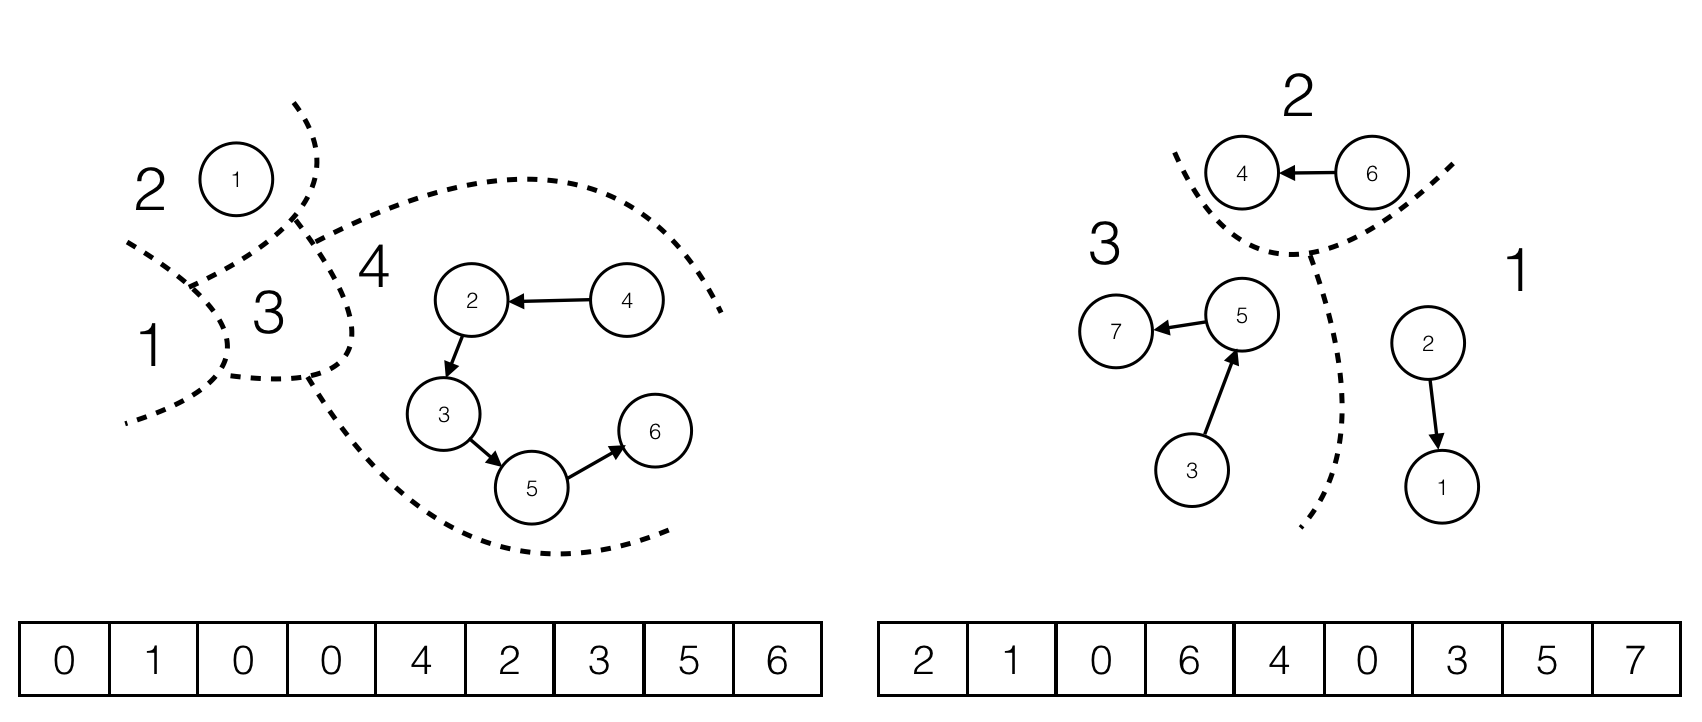
\includegraphics[width=0.7\textwidth]{distrito.png}
\vspace{0.5cm}
\caption{\label{fig:distrito}A esquerda um grafo com 6 nós e 2 distritos, sendo dois destes vazios. A direita um grafo com 7 nós e 3 distritos}
\end{figure}
    
    %\subsection{Crossover}
    
    %\subsection{Mutação}
    
    \section{Design do Sistema}
    
    Para o design do sistema composto do solver baseado em algoritmo genético, entidades (grafos, caminhos, etc) e ensaios foi utilizado a Linguagem de Modelagem Unificada (do inglês, UML - Unified Modeling Language) \cite{uml}. Foi utilizado quatro diagramas da UML para o design do projeto, sendo estes diagrama de requisitos, diagrama de pacotes, diagrama de classes e matriz de rastreabilidade.
    
    \subsection{Requisitos}
    
    A análise e especificação de requisitos de software envolve as atividades de determinar os objetivos de um software e as restrições associadas a ele. Ela deve também estabelecer o relacionamento entre estes objetivos e restrições e a especificação precisa do software\cite{leite}. Foram levantados três requisitos principais, modelagem das instâncias, processamento e análise dos resultados, conforme figura \ref{fig:UMLReq}.
    
\begin{figure}[H]
\centering
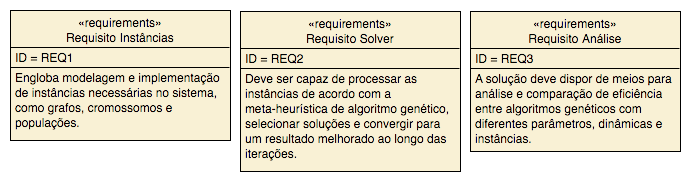
\includegraphics[width=0.9\textwidth]{UMLReq.png}
\vspace{0.5cm}
\caption{\label{fig:UMLReq}Diagrama de requisitos}
\end{figure}
    
    \subsection{Diagrama de Pacotes}
    
O diagrama de pacotes explicita as dependencias entre os pacotes que compõe o sistema \cite{uml}.
    
\begin{figure}[H]
\centering
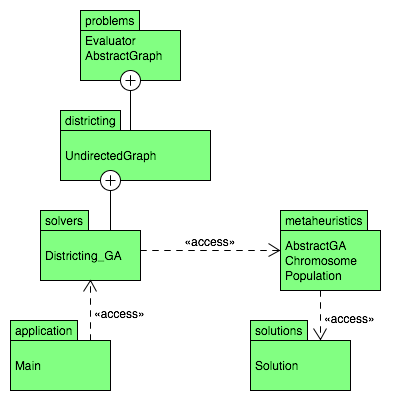
\includegraphics[width=0.7\textwidth]{UMLPkg.png}
\vspace{0.5cm}
\caption{\label{fig:UMLPkg}Diagrama de pacotes}
\end{figure}
    
    \subsection{Diagrama de Classes}
    
Um diagrama de classes no contexto da UML é um diagrama estruturado que descreve a morfologia de um sistema mostrando suas classes, atributos, operações (métodos) e as relações entre seus objetos \cite{classes}.
    
\begin{figure}[H]
\centering
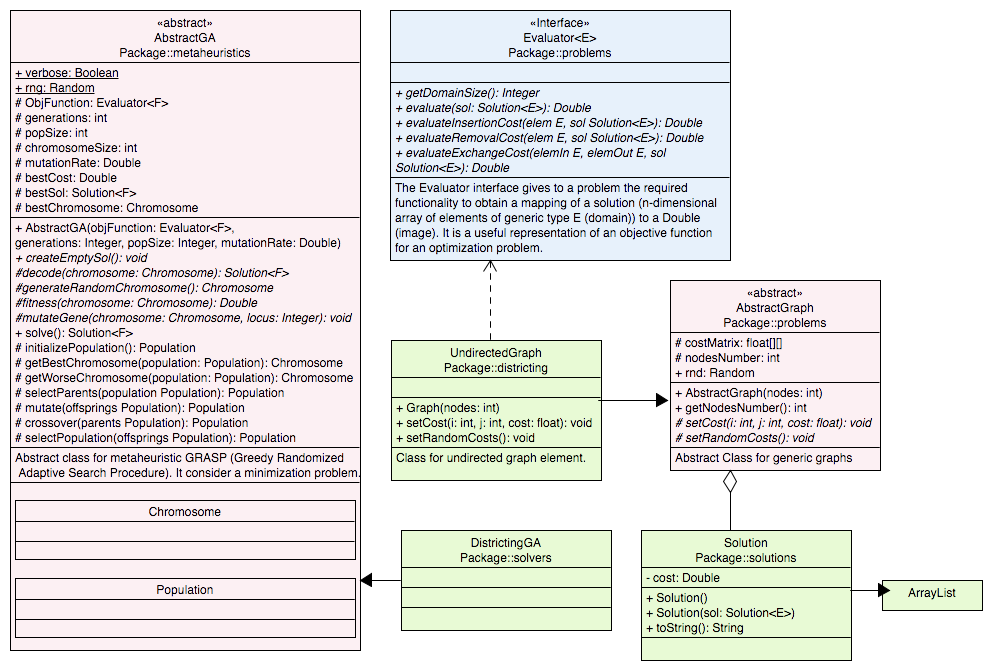
\includegraphics[width=1.1\textwidth]{UMLCasses.png}
\vspace{0.5cm}
\caption{\label{fig:UMLClasses}Diagrama de classes}
\end{figure}
    
    \subsection{Matriz de Rastreabilidade}
    
    A matriz de rastreabilidade de requisitos é um documento, usualmente na forma de tabela, usado para auxiliar na determinação da integridade de uma relação, correlacionando quaisquer dois documentos com base em uma comparação de relação muitos-para-muitos \cite{rast}. No nosso caso utilizamos a matriz de rastreabilidade para correlacionar as classes e métodos aos requisitos levantados.
    
\begin{table}[H]
\centering
\caption{Matriz de Rastreabilidade}
\vspace{0.5cm}
\label{rastreabilidade}
\begin{tabular}{|l|l|l|l|l|l|}
\hline
ID do Requisito 	& Implementação 	 	\\ \hline
REQ1		&    				\\ \hline
REQ2		&  					\\ \hline
REQ3		&  					\\ \hline
\end{tabular}
\end{table}
    
    
	\newpage
	\addcontentsline{toc}{section}{Referências}
	\bibliographystyle{model3-num-names}
    
    \section*{Referências}
    
	\begin{thebibliography}{1}
    
\bibitem{tang}
Shangce Gaoa, Yirui Wanga, Jiujun Chengc, Yasuhiro Inazumib, Zheng Tang. Ant colony optimization with clustering for solving the dynamic location routing problem. In: Ant colony algorithm, Clustering algorithm, Dynamic environment, Dynamic optimization Immigrant scheme, Location routing. Applied Mathematics and Computation 285 (2016) 149–173.

\bibitem{fernandez}
Gabriela Garcıa-Ayalaa, José Luis González-Velardea, Roger Z. Rios-Mercado and Elena Fernández. A novel model for arc territory design: promoting Eulerian districts. International Transactions in Operational Research 23 (2016) 433–458.

%\bibitem{laporte}
%Alexander Butsch, Jörg Kalcsics, Gilbert Laporte. Districting for Arc Routing. INFORMS Journal on Computing 26(4) (2014) 809-824.

\bibitem{prins}
Maria Cândida Mourão, Ana Catarina Nunes, Christian Prins. Heuristic methods for the sectoring arc routing problem. European Journal of Operational Research 196 (2009) 856–868.

\bibitem{wang}
Hongtao Lei, Rui Wang, Gilbert Laporte. Solving a multi-objective dynamic stochastic districting and routing problem with a co-evolutionary algorithm. Computers \& Operations Research 67 (2016) 12–24.

\bibitem{agarwal}
Agarwal, U., Singh, U.. Graph Theory. Laxmi Publications; 2009.

\bibitem{reeves}
Reeves, C.. Genetic Algorithms for the Operations Researcher. Journal on Computing Vol. 9, No.3, Summer 1997, 231 - 250.

\bibitem{groer}
Groër C, Golden BL, Wasil EA. The consistent vehicle routing problem. Manuf Serv Oper Manag 2009;11(4):630–43.

\bibitem{uml}
BOOCH, G; RUMBAUGH, J e JACOBSON, I: UML, Guia do Usuário: tradução; Fábio Freitas da Silva, Rio de Janeiro, Campus, 2012.

\bibitem{leite}
L, Jair C.. Notas de aula de Engenharia de Software . UFRN, 2001.

\bibitem{classes}
Goodwin, D.. Modelling and Simulation. University of Warwick, 2015.

\bibitem{rast}
Gotel, O., Cleland-Huang, J., Hayes, J. H., Zisman, A., Egyed, A., Grünbacher, P., Dekhtyar, A., Antoniol, G., Maletic, J. Software and Systems Traceability. Springer London pp. 3–22.

\bibitem{algoritmos}
CORMEN, T. H.; LEISERSON, C. E.; RIVEST, R. L. e STEIN, C. Introduction to Algorithms, 3a edição, MIT Press, 2009, p. 658-664.

	\end{thebibliography}
	
\end{document}